\begin{figure}

\caption{All plots}

\newlength{\plotwidth}
\setlength{\plotwidth}{0.33\textwidth}


\begin{subfigure}{1.0\textwidth}
\caption{Trial 2}
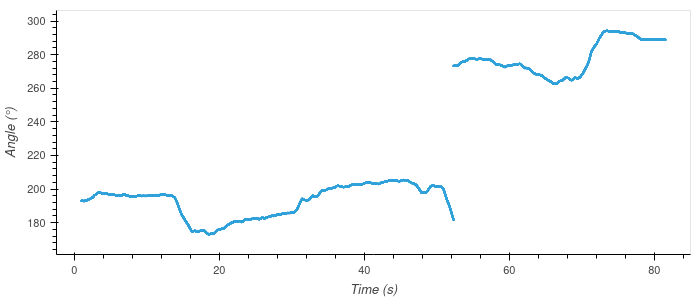
\includegraphics[width=\plotwidth]{plots/t2-time-angle.png}
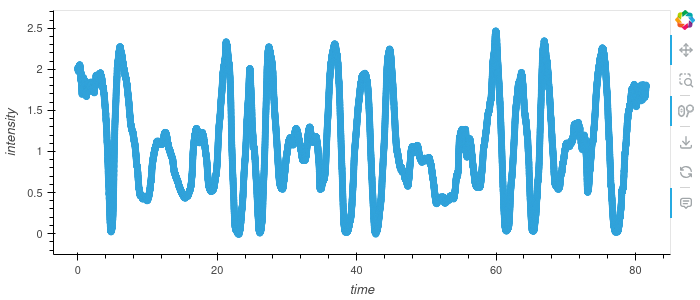
\includegraphics[width=\plotwidth]{plots/t2-time-intensity.png}
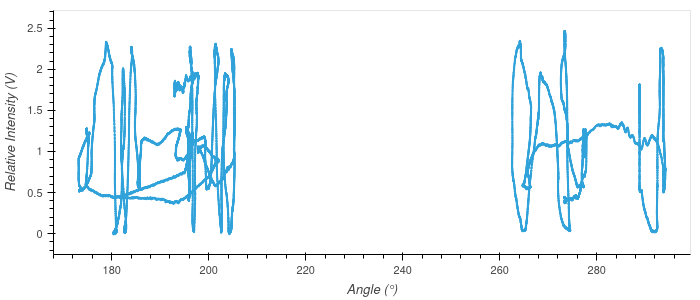
\includegraphics[width=\plotwidth]{plots/t2-angle-intensity.png}
\end{subfigure}



\begin{subfigure}{1.0\textwidth}
\caption{Trial 3}
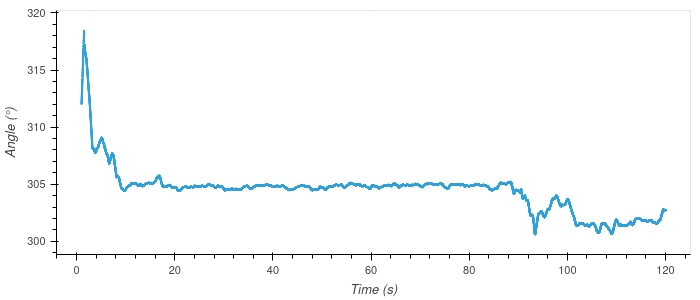
\includegraphics[width=\plotwidth]{plots/t3-time-angle.png}
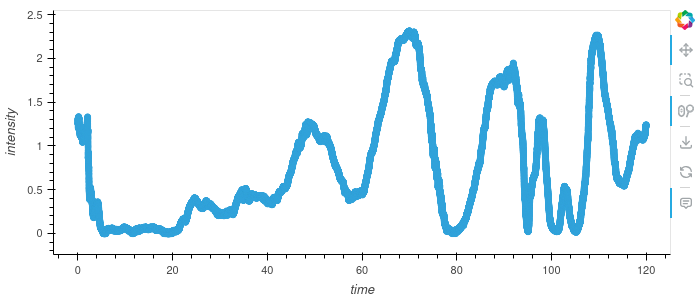
\includegraphics[width=\plotwidth]{plots/t3-time-intensity.png}
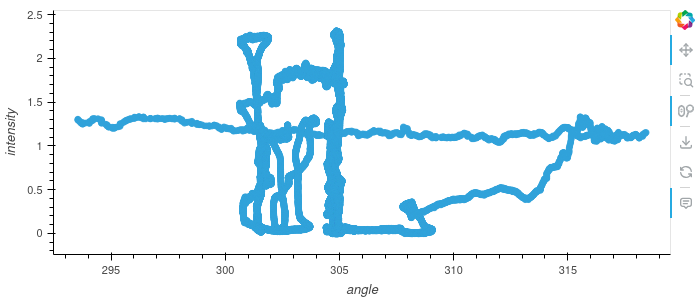
\includegraphics[width=\plotwidth]{plots/t3-angle-intensity.png}
\end{subfigure}



\begin{subfigure}{1.0\textwidth}
\caption{Trial 4}
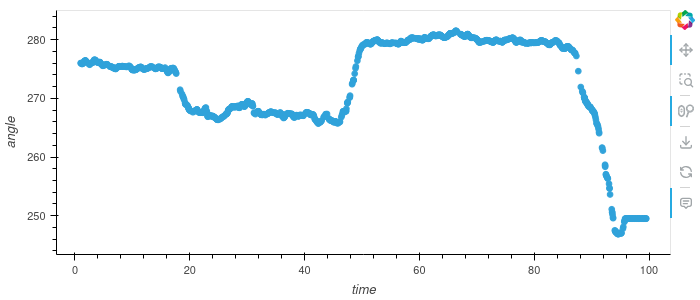
\includegraphics[width=\plotwidth]{plots/t4-time-angle.png}
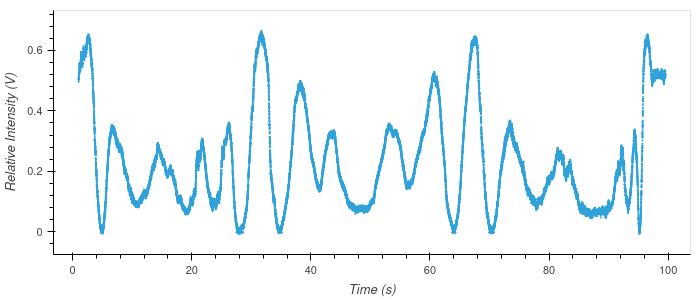
\includegraphics[width=\plotwidth]{plots/t4-time-intensity.png}
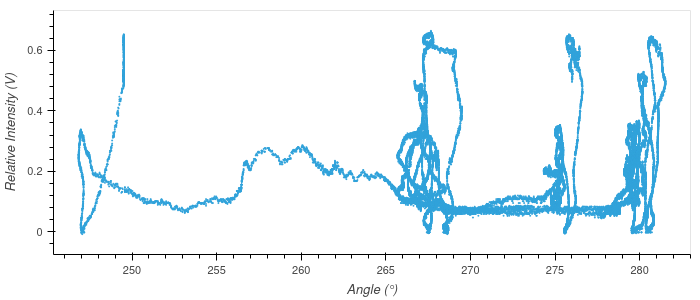
\includegraphics[width=\plotwidth]{plots/t4-angle-intensity.png}
\end{subfigure}



\begin{subfigure}{1.0\textwidth}
\caption{Trial 5}
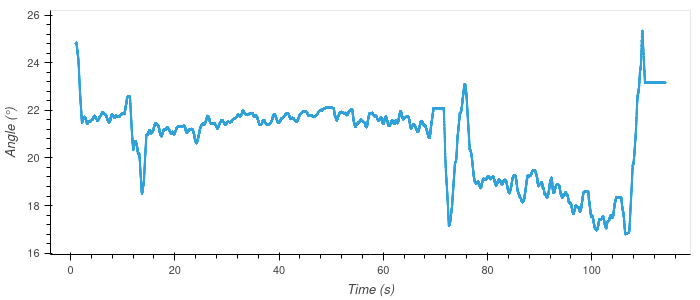
\includegraphics[width=\plotwidth]{plots/t6-time-angle.png}
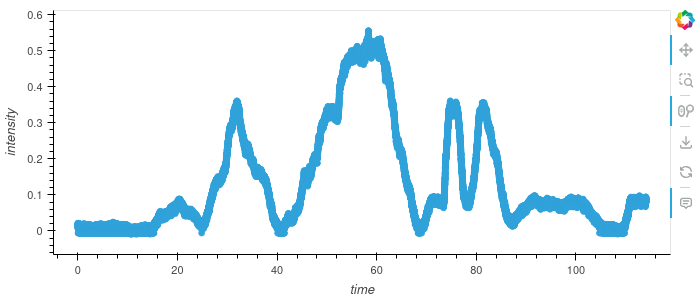
\includegraphics[width=\plotwidth]{plots/t6-time-intensity.png}
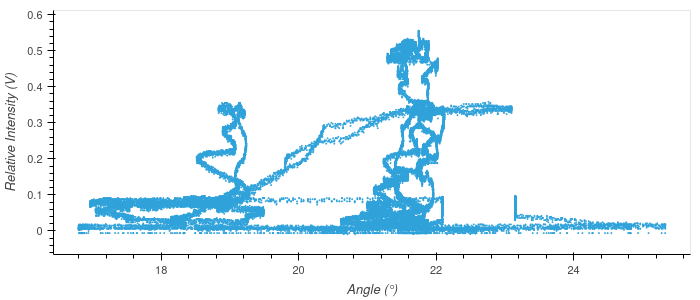
\includegraphics[width=\plotwidth]{plots/t6-angle-intensity.png}
\end{subfigure}



\begin{subfigure}{1.0\textwidth}
\caption{Trial 6}
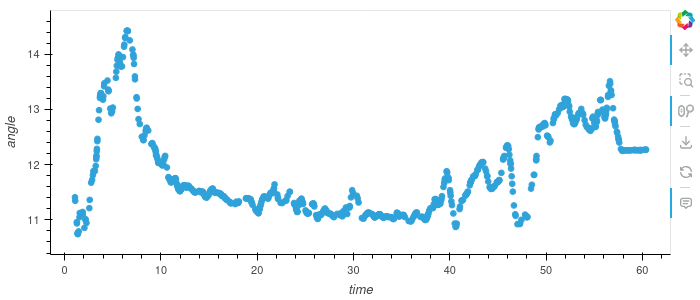
\includegraphics[width=\plotwidth]{plots/t7-time-angle.png}
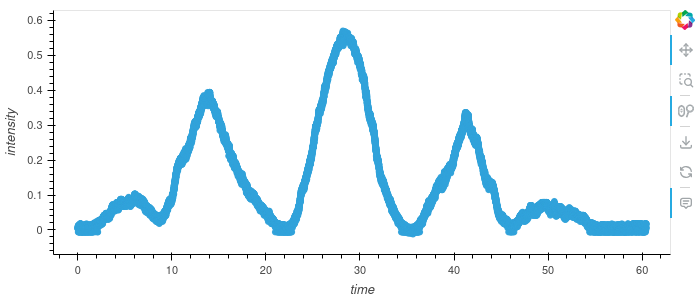
\includegraphics[width=\plotwidth]{plots/t7-time-intensity.png}
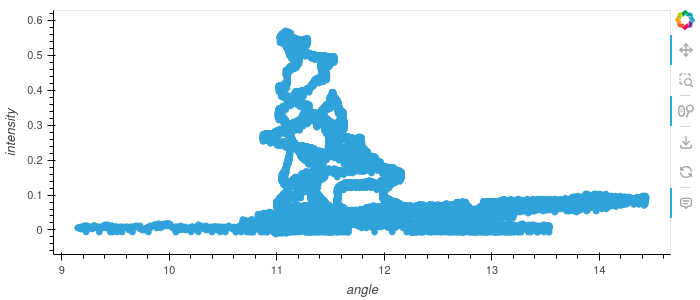
\includegraphics[width=\plotwidth]{plots/t7-angle-intensity.png}
\end{subfigure}



\begin{subfigure}{1.0\textwidth}
\caption{Trial 7}
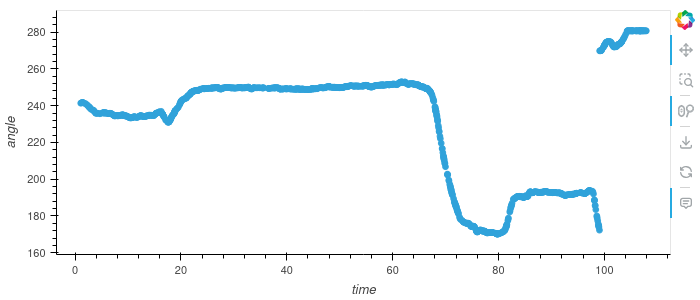
\includegraphics[width=\plotwidth]{plots/t8-time-angle.png}
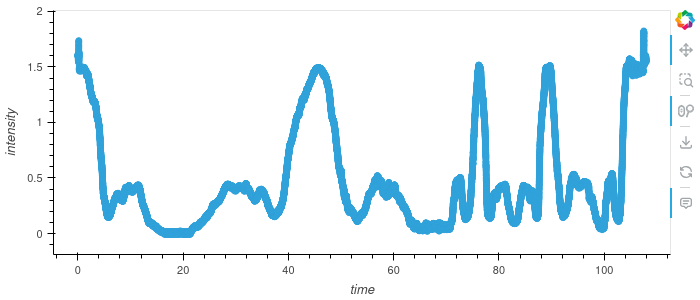
\includegraphics[width=\plotwidth]{plots/t8-time-intensity.png}
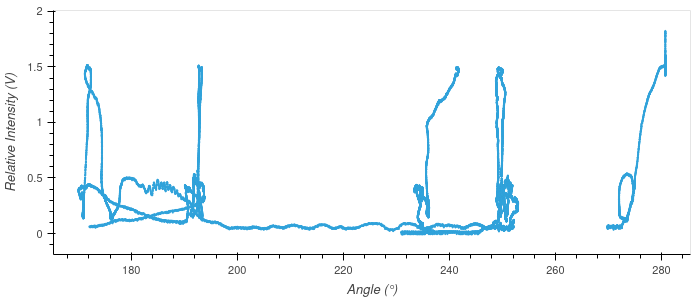
\includegraphics[width=\plotwidth]{plots/t8-angle-intensity.png}
\end{subfigure}

\caption*{
Left to right: time versus angle, time versus intensity, combined seres — angle versus intensity\\
Top to bottom: Trials 2 through 7
}
\end{figure}
